%#!platex main.tex
\chapter{序論}

\section{背景}
参考文献のテスト\cite{樋口龍雄2000}.
%"bibliography.bib"の中身をいじると変更できます.
正弦波の周波数推定はレーダーやソナー,通信,医療などの領域で幅広く研究されてきた課題である\cite{R.G.McKilliam,K.Wang,D.Rife}.
一般に,単一正弦波に対する周波数推定を行う場合,アナログ信号であれば周波数カウンタを用いる手法,ディジタル信号の場合,相関を用いた手法やヒルベルト変換器を用いる手法が提案されている.
周波数カウンタを用いた手法では,1周期に対して基準クロックを用いて測定し,その逆数から周波数を求めるレシプロカル方式の周波数カウンタが知られている.しかしこの手法を用いる場合,周波数が変化すると出力間隔が不等間隔になる.そのため,計測値に対して,ディジタル処理を行う場合には補完処理などの工夫が必要となるため,サンプルごとに周波数の推定値が出力されるヒルベルト変換器を用いた手法が提案されている.\\
 ヒルベルト変換器を用いた手法では,入力を実部,出力を虚部とする複素信号の一種である解析信号の位相を時間微分し,瞬時角周波数から瞬時周波数を推定することができる.従来,ヒルベルト変換器は有限次数のFIRフィルタとして設計されるため振幅特性にリプルが生じ,出力は振動する場合がある.高尾ら\cite{高尾可変なし,高尾可変あり}は振動成分の周波数が入力周波数の偶数倍であることを理論的に示し,これを伝送零点を有する可変FIRフィルタを用いて振動成分を除去することで,低次数なヒルベルト変換器を用いても,単一正弦波の高精度な瞬時周波数推定が可能となることを示した.
%高尾さんのやつと関連させてノイズを取れることを書きたいなら,どういうノイズが取れて,どういうノイズがダメなのか明記する必要がある.
しかし実際にはノイズを含む信号を解析する必要がある.一般に,ノイズを含む信号に対して,ヒルベルト変換を行うためには,あらかじめ帯域通過フィルタによりノイズを低減させた後に,ヒルベルト変換器を縦続接続する方法が考えられる.しかし,帯域通過フィルタとヒルベルト変換器を1つのフィルタとして見た場合,全体の次数が増加し,結果として遅延や回路規模の増大につながり好ましくない.\\
 そこで本稿では,阻止域を有するヒルベルト変換器に対し,指定した位置に伝送零点を置くことで,ノイズを除去しながらヒルベルト変換可能なフィルタを設計する.阻止域を有するヒルベルト変換器を設計する場合,本来であれば阻止域において十分な減衰量を確保するために多くのフィルタ次数が必要となる.しかし,特定の周波数成分にノイズが含まれることがわかっている場合,その周波数成分のみに伝送零点を入れることにより,特定のノイズのみ除去しながらヒルベルト変換を行うことができ,減衰量を確保するために必要な次数を削減することができる.
最後に設計例を示し,提案法の有効性を確認する.
\section{目的}
本章では提案するフィルタの設計問題について記す.提案するフィルタは,阻止域の指定した位置に伝送零点を有するヒルベルト変換器である.本稿で設計するフィルタの振幅理想特性を図\ref{ideal_resp}に示す.またフィルタの振幅理想特性は正規化角周波数$\omega$を用いて,

\begin{figure}[tb]
    \centering
    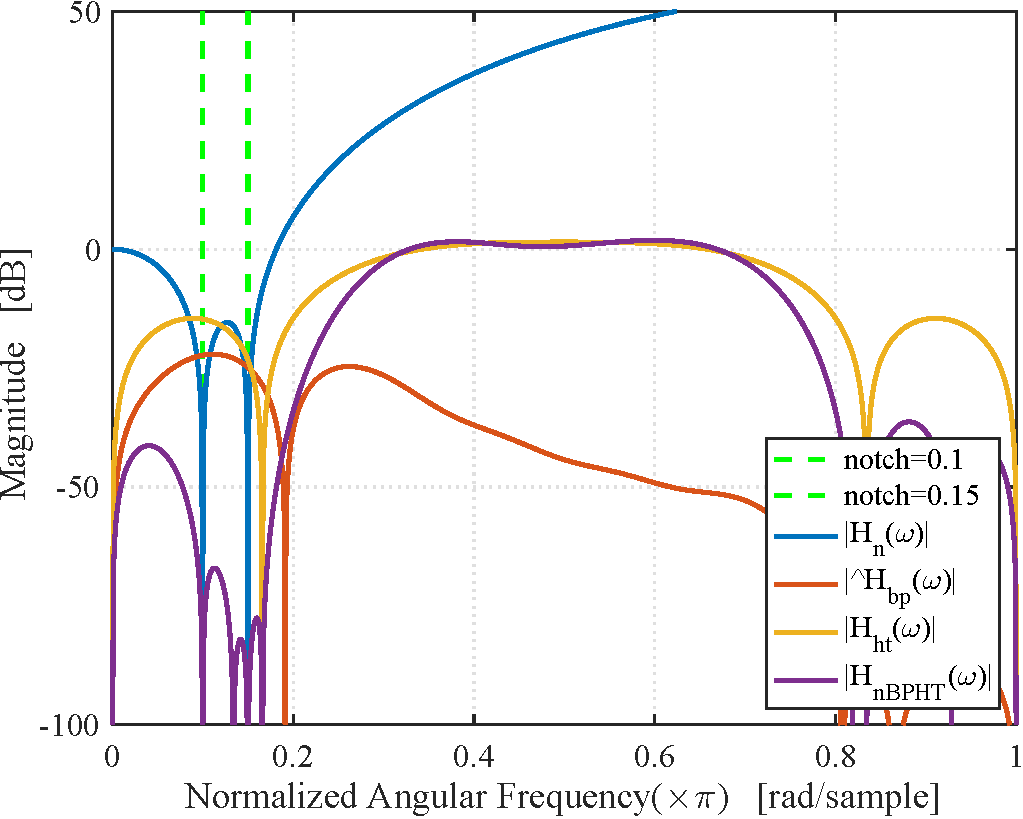
\includegraphics[width=8cm]
    		{Figure/figure01.pdf}
    \caption{}
    \label{fig:man}
\end{figure}